\documentclass[tikz,border=5pt]{standalone}
\usepackage{amsmath}
\usepackage[T1]{fontenc}
\usetikzlibrary{arrows,calc,positioning}

\definecolor{dataBlue}{HTML}{4C78A8}
\definecolor{baselineGray}{HTML}{8C8C8C}
\definecolor{residualAmber}{HTML}{E08E2B}
\definecolor{scalarTeal}{HTML}{2A9D8F}
\definecolor{predictionGreen}{HTML}{59A14F}
\definecolor{charcoal}{HTML}{3A3A3A}

\begin{document}
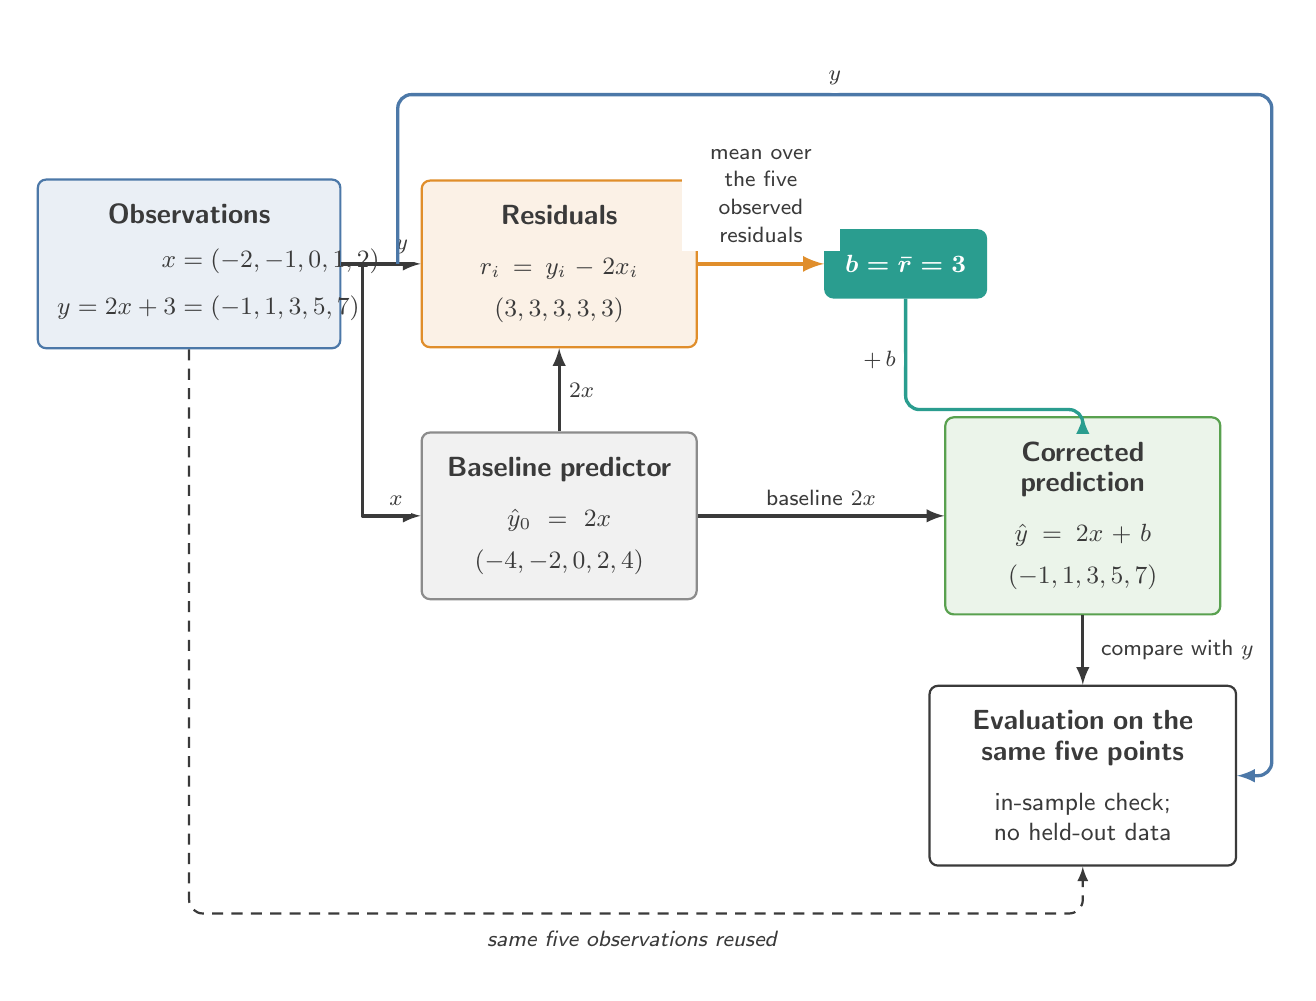
\begin{tikzpicture}[
    font=\sffamily\fontsize{9}{11}\selectfont,
    text=charcoal,
    box/.style={
        rectangle,
        rounded corners=3pt,
        line width=0.8pt,
        align=center,
        inner xsep=7pt,
        inner ysep=9pt
    },
    flow/.style={
        -latex,
        line width=1.2pt,
        draw=charcoal,
        line join=round
    },
    dependency/.style={
        flow,
        line width=1.6pt,
        draw=residualAmber
    },
    reuse/.style={
        -latex,
        dashed,
        dash pattern=on 4pt off 3pt,
        line width=0.8pt,
        draw=charcoal,
        rounded corners=5pt
    },
    label/.style={
        font=\sffamily\fontsize{8}{10}\selectfont,
        align=center,
        fill=white,
        inner sep=3pt
    },
    header/.style={
        font=\sffamily\bfseries\fontsize{10}{12}\selectfont
    }
]

% White 4:3 canvas.
\path[use as bounding box,fill=white] (0,0) rectangle (16,12);

% Observations.
\node[box,draw=dataBlue,fill=dataBlue!12,text width=3.35cm]
    (D1) at (2.05,9.0) {
    {\bfseries\fontsize{10}{12}\selectfont Observations}\\[7pt]
    \(\begin{aligned}
        x&=(-2,-1,0,1,2)\\[3pt]
        y=2x+3&=(-1,1,3,5,7)
    \end{aligned}\)
};

% Computation.
\node[box,draw=baselineGray,fill=baselineGray!12,text width=3.0cm]
    (B) at (6.75,5.8) {
    {\bfseries\fontsize{10}{12}\selectfont Baseline predictor}\\[7pt]
    \(\hat y_0=2x\)\\[4pt]
    \((-4,-2,0,2,4)\)
};

\node[box,draw=residualAmber,fill=residualAmber!12,text width=3.0cm]
    (R) at (6.75,9.0) {
    {\bfseries\fontsize{10}{12}\selectfont Residuals}\\[7pt]
    \(r_i=y_i-2x_i\)\\[4pt]
    \((3,3,3,3,3)\)
};

% The only saturated-fill node.
\node[box,draw=scalarTeal,fill=scalarTeal,
      text=white,text width=1.55cm,minimum height=0.85cm]
    (S) at (11.15,9.0) {
    \(\boldsymbol{b=\bar r=3}\)
};

% Corrected prediction and evaluation.
\node[box,draw=predictionGreen,fill=predictionGreen!12,
      text width=3.0cm]
    (C) at (13.4,5.8) {
    {\bfseries\fontsize{10}{12}\selectfont Corrected prediction}\\[7pt]
    \(\hat y=2x+b\)\\[4pt]
    \((-1,1,3,5,7)\)
};

\node[box,draw=charcoal,fill=white,text width=3.4cm]
    (E) at (13.4,2.5) {
    {\bfseries\fontsize{10}{12}\selectfont
     Evaluation on the\\same five points}\\[7pt]
    in-sample check;\\
    no held-out data
};

% One shared observation output, branching into x and y.
\coordinate (split) at (4.25,9.0);
\coordinate (targetbranch) at (4.7,9.0);
\draw[line width=1.2pt,draw=charcoal] (D1.east) -- (split);

\draw[flow]
    (split) -- (4.25,5.8)
    -- node[label,above,pos=0.58] {\(x\)} (B.west);

\draw[flow]
    (split) -- node[label,above,pos=0.68] {\(y\)} (R.west);

% Baseline contribution to the observed residuals.
\draw[flow]
    (B.north) -- node[label,right] {\(2x\)} (R.south);

% Emphasized observed-residual-to-scalar dependency.
\draw[dependency]
    (R.east) --
    node[label,above=4pt,text width=1.8cm] {
        mean over the five\\observed residuals
    }
    (S.west);

% Combine the baseline and scalar correction.
\draw[flow]
    (B.east) --
    node[label,above] {baseline \(2x\)}
    (C.west);

\draw[flow,draw=scalarTeal,rounded corners=5pt]
    (S.south) --
    node[label,left,pos=0.55] {\(+\,b\)}
    (11.15,7.15) -- (13.4,7.15) -- (C.north);

% Prediction enters the evaluation.
\draw[flow]
    (C.south) --
    node[label,right=3pt] {compare with \(y\)}
    (E.north);

% Explicit target input to evaluation, routed around the upper/right margin.
\draw[flow,draw=dataBlue,rounded corners=5pt]
    (targetbranch) -- (4.7,11.15)
    -- node[label,above] {\(y\)}
    (15.8,11.15) -- (15.8,2.5) -- (E.east);

% Separate lower-margin reuse dependency.
\draw[reuse]
    (D1.south) -- (2.05,0.75)
    -- node[label,below=3pt,
            font=\sffamily\itshape\fontsize{8}{10}\selectfont] {
        same five observations reused
    }
    (13.4,0.75) -- (E.south);

\end{tikzpicture}
\end{document}